% Options for packages loaded elsewhere
\PassOptionsToPackage{unicode}{hyperref}
\PassOptionsToPackage{hyphens}{url}
%
\documentclass[
  ignorenonframetext,
  t]{beamer}
\usepackage{pgfpages}
\setbeamertemplate{caption}[numbered]
\setbeamertemplate{caption label separator}{: }
\setbeamercolor{caption name}{fg=normal text.fg}
\beamertemplatenavigationsymbolsempty
% Prevent slide breaks in the middle of a paragraph
\widowpenalties 1 10000
\raggedbottom
\setbeamertemplate{part page}{
  \centering
  \begin{beamercolorbox}[sep=16pt,center]{part title}
    \usebeamerfont{part title}\insertpart\par
  \end{beamercolorbox}
}
\setbeamertemplate{section page}{
  \centering
  \begin{beamercolorbox}[sep=12pt,center]{part title}
    \usebeamerfont{section title}\insertsection\par
  \end{beamercolorbox}
}
\setbeamertemplate{subsection page}{
  \centering
  \begin{beamercolorbox}[sep=8pt,center]{part title}
    \usebeamerfont{subsection title}\insertsubsection\par
  \end{beamercolorbox}
}
\AtBeginPart{
  \frame{\partpage}
}
\AtBeginSection{
  \ifbibliography
  \else
    \frame{\sectionpage}
  \fi
}
\AtBeginSubsection{
  \frame{\subsectionpage}
}
\usepackage{lmodern}
\usepackage{amssymb,amsmath}
\usepackage{ifxetex,ifluatex}
\ifnum 0\ifxetex 1\fi\ifluatex 1\fi=0 % if pdftex
  \usepackage[T1]{fontenc}
  \usepackage[utf8]{inputenc}
  \usepackage{textcomp} % provide euro and other symbols
\else % if luatex or xetex
  \usepackage{unicode-math}
  \defaultfontfeatures{Scale=MatchLowercase}
  \defaultfontfeatures[\rmfamily]{Ligatures=TeX,Scale=1}
\fi
\usecolortheme{spruce}
\usefonttheme{serif}
% Use upquote if available, for straight quotes in verbatim environments
\IfFileExists{upquote.sty}{\usepackage{upquote}}{}
\IfFileExists{microtype.sty}{% use microtype if available
  \usepackage[]{microtype}
  \UseMicrotypeSet[protrusion]{basicmath} % disable protrusion for tt fonts
}{}
\makeatletter
\@ifundefined{KOMAClassName}{% if non-KOMA class
  \IfFileExists{parskip.sty}{%
    \usepackage{parskip}
  }{% else
    \setlength{\parindent}{0pt}
    \setlength{\parskip}{6pt plus 2pt minus 1pt}}
}{% if KOMA class
  \KOMAoptions{parskip=half}}
\makeatother
\usepackage{xcolor}
\IfFileExists{xurl.sty}{\usepackage{xurl}}{} % add URL line breaks if available
\IfFileExists{bookmark.sty}{\usepackage{bookmark}}{\usepackage{hyperref}}
\hypersetup{
  pdftitle={Associations},
  hidelinks,
  pdfcreator={LaTeX via pandoc}}
\urlstyle{same} % disable monospaced font for URLs
\newif\ifbibliography
\usepackage{color}
\usepackage{fancyvrb}
\newcommand{\VerbBar}{|}
\newcommand{\VERB}{\Verb[commandchars=\\\{\}]}
\DefineVerbatimEnvironment{Highlighting}{Verbatim}{commandchars=\\\{\}}
% Add ',fontsize=\small' for more characters per line
\usepackage{framed}
\definecolor{shadecolor}{RGB}{248,248,248}
\newenvironment{Shaded}{\begin{snugshade}}{\end{snugshade}}
\newcommand{\AlertTok}[1]{\textcolor[rgb]{0.94,0.16,0.16}{#1}}
\newcommand{\AnnotationTok}[1]{\textcolor[rgb]{0.56,0.35,0.01}{\textbf{\textit{#1}}}}
\newcommand{\AttributeTok}[1]{\textcolor[rgb]{0.77,0.63,0.00}{#1}}
\newcommand{\BaseNTok}[1]{\textcolor[rgb]{0.00,0.00,0.81}{#1}}
\newcommand{\BuiltInTok}[1]{#1}
\newcommand{\CharTok}[1]{\textcolor[rgb]{0.31,0.60,0.02}{#1}}
\newcommand{\CommentTok}[1]{\textcolor[rgb]{0.56,0.35,0.01}{\textit{#1}}}
\newcommand{\CommentVarTok}[1]{\textcolor[rgb]{0.56,0.35,0.01}{\textbf{\textit{#1}}}}
\newcommand{\ConstantTok}[1]{\textcolor[rgb]{0.00,0.00,0.00}{#1}}
\newcommand{\ControlFlowTok}[1]{\textcolor[rgb]{0.13,0.29,0.53}{\textbf{#1}}}
\newcommand{\DataTypeTok}[1]{\textcolor[rgb]{0.13,0.29,0.53}{#1}}
\newcommand{\DecValTok}[1]{\textcolor[rgb]{0.00,0.00,0.81}{#1}}
\newcommand{\DocumentationTok}[1]{\textcolor[rgb]{0.56,0.35,0.01}{\textbf{\textit{#1}}}}
\newcommand{\ErrorTok}[1]{\textcolor[rgb]{0.64,0.00,0.00}{\textbf{#1}}}
\newcommand{\ExtensionTok}[1]{#1}
\newcommand{\FloatTok}[1]{\textcolor[rgb]{0.00,0.00,0.81}{#1}}
\newcommand{\FunctionTok}[1]{\textcolor[rgb]{0.00,0.00,0.00}{#1}}
\newcommand{\ImportTok}[1]{#1}
\newcommand{\InformationTok}[1]{\textcolor[rgb]{0.56,0.35,0.01}{\textbf{\textit{#1}}}}
\newcommand{\KeywordTok}[1]{\textcolor[rgb]{0.13,0.29,0.53}{\textbf{#1}}}
\newcommand{\NormalTok}[1]{#1}
\newcommand{\OperatorTok}[1]{\textcolor[rgb]{0.81,0.36,0.00}{\textbf{#1}}}
\newcommand{\OtherTok}[1]{\textcolor[rgb]{0.56,0.35,0.01}{#1}}
\newcommand{\PreprocessorTok}[1]{\textcolor[rgb]{0.56,0.35,0.01}{\textit{#1}}}
\newcommand{\RegionMarkerTok}[1]{#1}
\newcommand{\SpecialCharTok}[1]{\textcolor[rgb]{0.00,0.00,0.00}{#1}}
\newcommand{\SpecialStringTok}[1]{\textcolor[rgb]{0.31,0.60,0.02}{#1}}
\newcommand{\StringTok}[1]{\textcolor[rgb]{0.31,0.60,0.02}{#1}}
\newcommand{\VariableTok}[1]{\textcolor[rgb]{0.00,0.00,0.00}{#1}}
\newcommand{\VerbatimStringTok}[1]{\textcolor[rgb]{0.31,0.60,0.02}{#1}}
\newcommand{\WarningTok}[1]{\textcolor[rgb]{0.56,0.35,0.01}{\textbf{\textit{#1}}}}
\setlength{\emergencystretch}{3em} % prevent overfull lines
\providecommand{\tightlist}{%
  \setlength{\itemsep}{0pt}\setlength{\parskip}{0pt}}
\setcounter{secnumdepth}{-\maxdimen} % remove section numbering
\usepackage{tabto}
\usepackage{verbatim}
\usepackage{amsmath}
\usepackage{mathtools}
\usepackage{graphicx}
\usepackage{tikz}
\usepackage{tikzpagenodes}
\definecolor{OG}{RGB}{0,64,8}
\definecolor{LG}{RGB}{0,102,51}
\definecolor{myRed}{RGB}{228,26,28}
\definecolor{myBlue}{RGB}{55,126,184}
\definecolor{myGreen}{RGB}{77,175,74}
\definecolor{myPurple}{RGB}{152,78,163}
\setbeamercolor{itemize item}{fg=white!0!LG}
\setbeamercolor{enumerate item}{fg=white!0!LG}
\setbeamercolor{enumerate subitem}{fg=white!70!LG}
\setbeamercolor{itemize subitem}{fg=white!70!LG}
\setbeamercolor{itemize subsubitem}{fg=white!70!LG}
\setbeamercolor{navigation symbols}{fg=white!70!LG, bg=white!70!LG}
\usepackage{inputenc}
\usepackage{booktabs}
\usepackage{caption}
\usetikzlibrary{patterns,arrows,decorations.pathreplacing}
\usepackage{setspace}
\DeclareGraphicsExtensions{.pdf,.png,.jpg,.gif}
\usepackage{fixmath}
\usepackage{tabto}
\usepackage{arydshln}
\textbackslash graphicspath\{``C:/Users/megha/Box/Courses/NRC\_290b\_2019\_Fall/Images/Assoc/''\}

\title{Associations}
\author{Introduction to Quantitative Ecology\\
Fall 2018\\
Chris Sutherland\\
\href{mailto:csutherland@umass.edu}{\nolinkurl{csutherland@umass.edu}}}
\date{}

\begin{document}
\frame{\titlepage}

\begin{frame}{Group evaluations}
\protect\hypertarget{group-evaluations}{}

\vfill

\begin{enumerate}
\tightlist
\item
  Specifically for the assignment due tomorrow, how would you describe
  your comfort levels with R and Excel?
\end{enumerate}

\begin{enumerate}[\hspace{0.5cm}A.]
  \item[A)] Uncomfortable with both
  \item[B)] Comfortable with Excel, but not R
  \item[C)] Comfortable with R, but not Excel
  \item[D)] Comfortable with both
\end{enumerate}

\begin{tikzpicture}[remember picture,overlay]
\node[xshift=-2cm,yshift=1cm] at (current page.south east)
{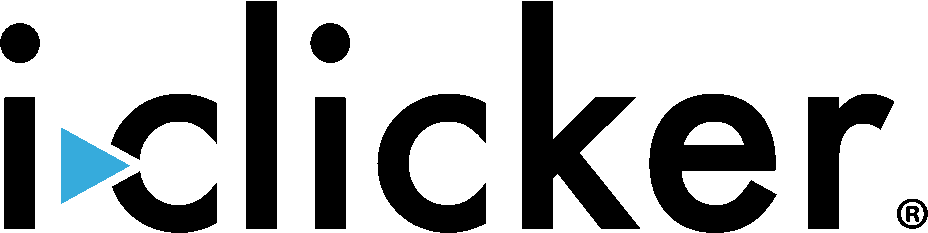
\includegraphics[height=0.25in]{iclicker.png}};
\end{tikzpicture}

\vfill

\end{frame}

\begin{frame}{One Question}
\protect\hypertarget{one-question}{}

\vfill

\begin{enumerate}
\tightlist
\item
  If you were using Pearson's residuals to see which specific
  associations in a contingency table were likely to be significant,
  which of the following values would be the critical value to use?
\end{enumerate}

\begin{enumerate}[\hspace{0.5cm}A.]
  \item[A)] 3.84
  \item[B)] -2 and 2
  \item[C)] 0.05
  \item[D)] 10/25/1980
\end{enumerate}

\vfill

\begin{tikzpicture}[remember picture,overlay]
\node[xshift=-2cm,yshift=1cm] at (current page.south east)
{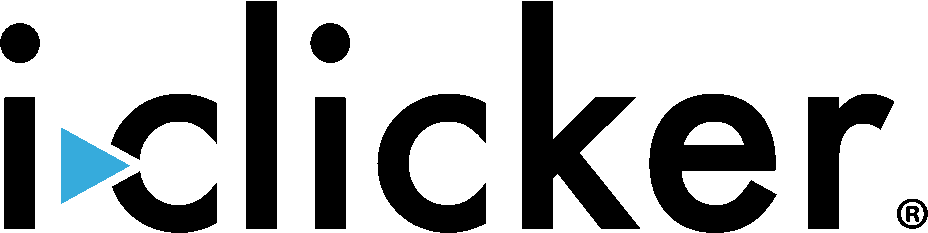
\includegraphics[height=0.25in]{iclicker.png}};
\end{tikzpicture}

\end{frame}

\begin{frame}{Group evaluations}
\protect\hypertarget{group-evaluations-1}{}

Is there a significant association between salamander \emph{sex} and
\emph{habitat type}?

\[\chi^2 = \sum \frac{(\text{Obs} - \text{Exp})^2}{\text{Exp}}\]

\begin{enumerate}
\tightlist
\item
  Calculate \(\chi^2\).\\
\item
  Calculate \(DF\)\\
\item
  Is there a significant association?
\end{enumerate}

\vspace{1cm}

\begin{tabular}{lcccc}
\hline     
           & Dry & Moist & Wet & $\sum$ Row \\ 
\hline
Female     & \emph{370} & \emph{198} & \emph{187} &      \\   
Male       & \emph{359} & \emph{110} & \emph{160} &      \\ 
$\sum$ Col &       &         &       &      \\ 
\hline
\end{tabular}

\begin{tikzpicture}[remember picture,overlay]
\node[xshift=-2cm,yshift=-1.5cm] at (current page.east)
{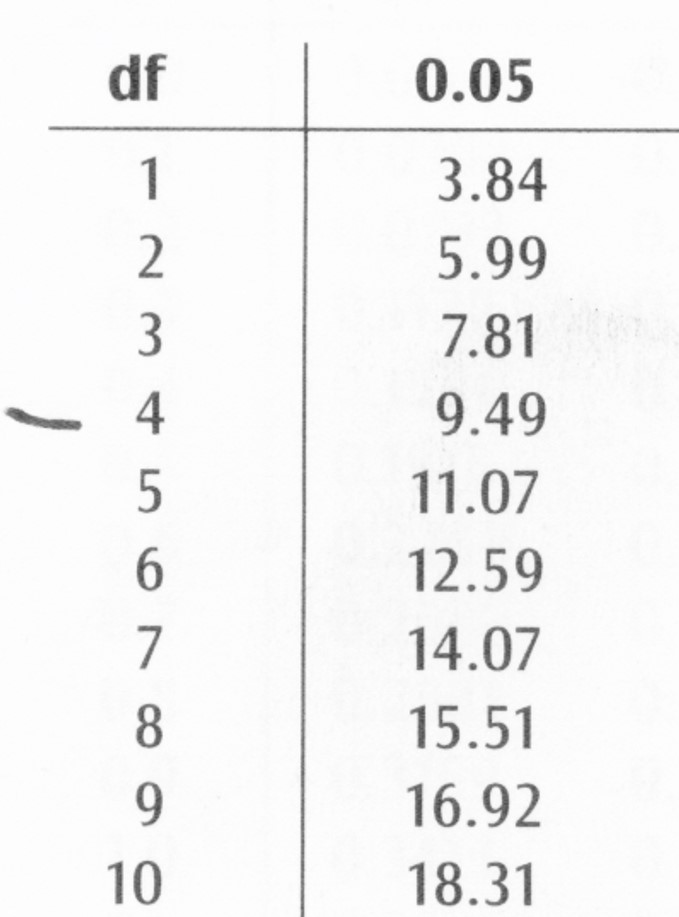
\includegraphics[height=1.75in]{chiTab.jpg}};
\end{tikzpicture}

\end{frame}

\begin{frame}{Associations}
\protect\hypertarget{associations}{}

What are associations?

\begin{itemize}
\tightlist
\item
  dealing with two categorical variables
\item
  known as a \emph{contingency table}

  \begin{itemize}
  \tightlist
  \item
    data are \emph{cross tabulated} frequencies
  \item
    each cell represents a count
  \end{itemize}
\end{itemize}

\end{frame}

\begin{frame}{Associations}
\protect\hypertarget{associations-1}{}

\begin{itemize}
\tightlist
\item
  dealing with two categorical variables
\item
  known as a \emph{contingency table}

  \begin{itemize}
  \tightlist
  \item
    data are \emph{cross tabulated} frequencies
  \item
    each cell represents a count
  \end{itemize}
\end{itemize}

\vspace{0.5cm}

\centering

\begin{tabular}{lccc}
\hline     
Salamander & Upland & Wetland & Floodplain \\ \hline
Present    & \emph{38}    & \emph{30} & \emph{24} \\   
Absent   & \emph{12}    & \emph{20} & \emph{26} \\ 
\hline
\end{tabular}

\vspace{1cm}

\end{frame}

\begin{frame}{Associations}
\protect\hypertarget{associations-2}{}

\begin{itemize}
\tightlist
\item
  dealing with two categorical variables
\item
  known as a \emph{contingency table}

  \begin{itemize}
  \tightlist
  \item
    data are \emph{cross tabulated} frequencies
  \item
    each cell represents a count
  \end{itemize}
\item
  visualize using a \emph{bar chart}
\end{itemize}

\scriptsize

\begin{tikzpicture}[remember picture,overlay]
\node[xshift=0cm,yshift=2.5cm] at (current page.south)
{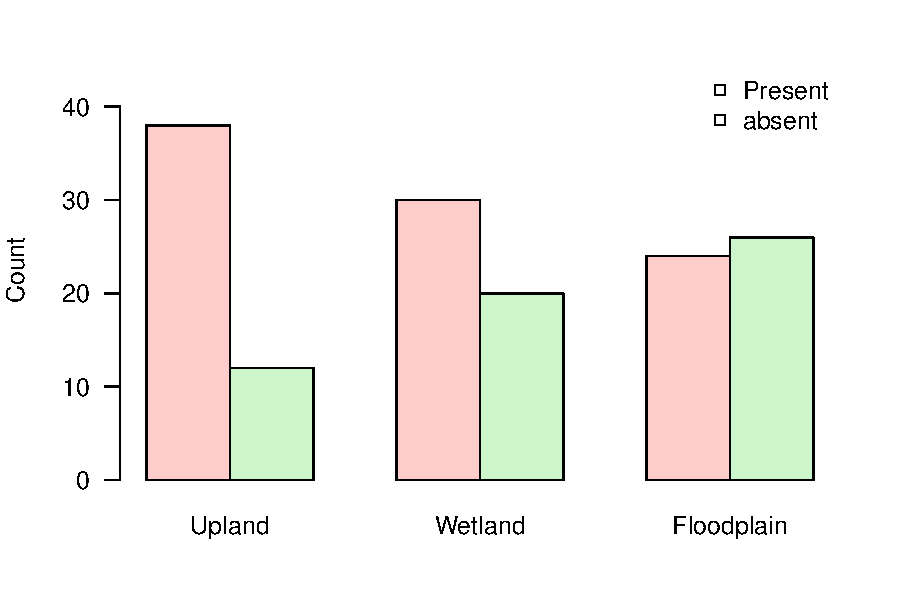
\includegraphics[height=2in]{manderContTab.pdf}};
\end{tikzpicture}

\end{frame}

\begin{frame}{Associations}
\protect\hypertarget{associations-3}{}

The key question with contingency tables:

\begin{itemize}
\tightlist
\item
  is there a significant association between the categorical variable A
  and categorical variable B?
\item
  are these numbers different to what we would expect to see by chance?
\end{itemize}

\end{frame}

\begin{frame}{Associations}
\protect\hypertarget{associations-4}{}

The key question with contingency tables:

\begin{itemize}
\tightlist
\item
  is there a significant association between the categorical variable A
  and categorical variable B?
\item
  are these number different to what we would expect to see by chance?
\item
  answer using the \emph{Chi-squared test}
\end{itemize}

\[ \chi^2 = \sum \frac{(O-E)^2}{E}\]

\begin{itemize}
\tightlist
\item
  O: the observed data
\item
  E: the expected value if there was \emph{no association}
\item
  \(\chi^2\): the test statistic
\end{itemize}

\end{frame}

\begin{frame}{Associations}
\protect\hypertarget{associations-5}{}

In a Chi-squared test from the following contingency table, I get a test
statistic of \(\chi^2 = 8.32\). Is there a significant association
between spotted salamander presence and vernal pool type at the 5\%
level?

\vspace{0.5cm}

\centering

\begin{tabular}{lccc}
\hline     
Salamander & Upland & Wetland & Floodplain \\ \hline
Present    & \emph{38}    & \emph{30} & \emph{24} \\   
Absent   & \emph{12}    & \emph{20} & \emph{26} \\ 
\hline
\end{tabular}

\vspace{1cm}

\begin{enumerate}[\hspace{0.5cm}A.]
  \item[A)] Yes, its significant!
  \item[B)] No, it's not significant!
\end{enumerate}

\begin{tikzpicture}[remember picture,overlay]
\node[xshift=-2cm,yshift=2cm] at (current page.south east)
{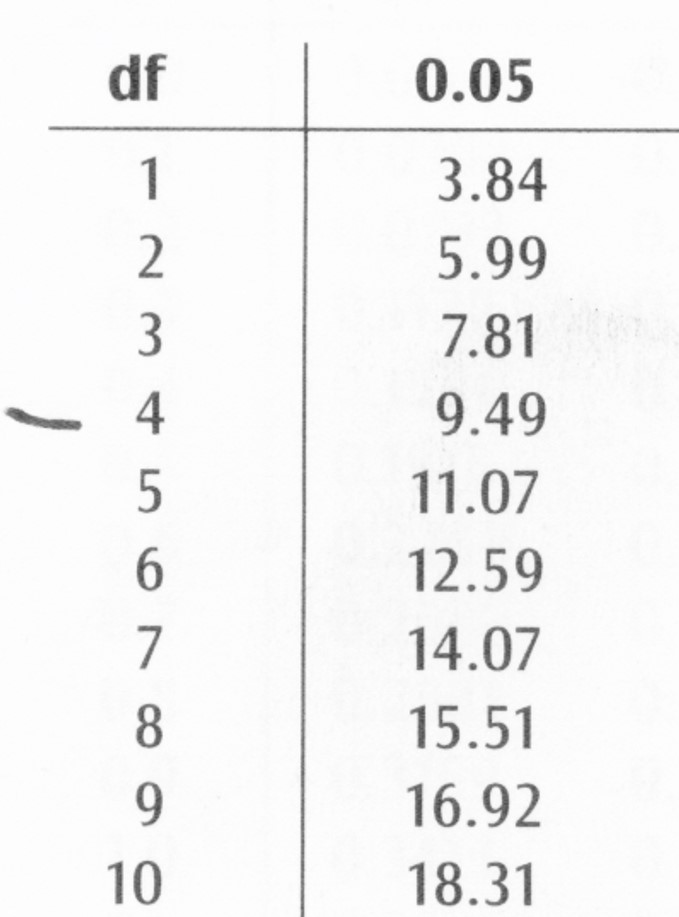
\includegraphics[height=1.4in]{chiTab.jpg}};
\end{tikzpicture}

\end{frame}

\begin{frame}{Associations}
\protect\hypertarget{associations-6}{}

In a Chi-squared test from the following contingency table, I get a test
statistic of \(\chi^2 = 8.32\). Is there a significant association
between spotted salamander presence and vernal pool type at the 5\%
level?

\vspace{0.5cm}

\centering

\begin{tabular}{lccc}
\hline     
Salamander & Upland & Wetland & Floodplain \\ \hline
Present    & \emph{38}    & \emph{30} & \emph{24} \\   
Absent   & \emph{12}    & \emph{20} & \emph{26} \\ 
\hline
\end{tabular}

\vspace{1cm}

\begin{enumerate}[\hspace{0.5cm}A.]
  \item[A)] \textbf{Yes, its significant!}
  \item[B)] \textcolor{gray}{No, it's not significant!}
\end{enumerate}

\begin{tikzpicture}[remember picture,overlay]
\node[xshift=-2cm,yshift=2cm] at (current page.south east)
{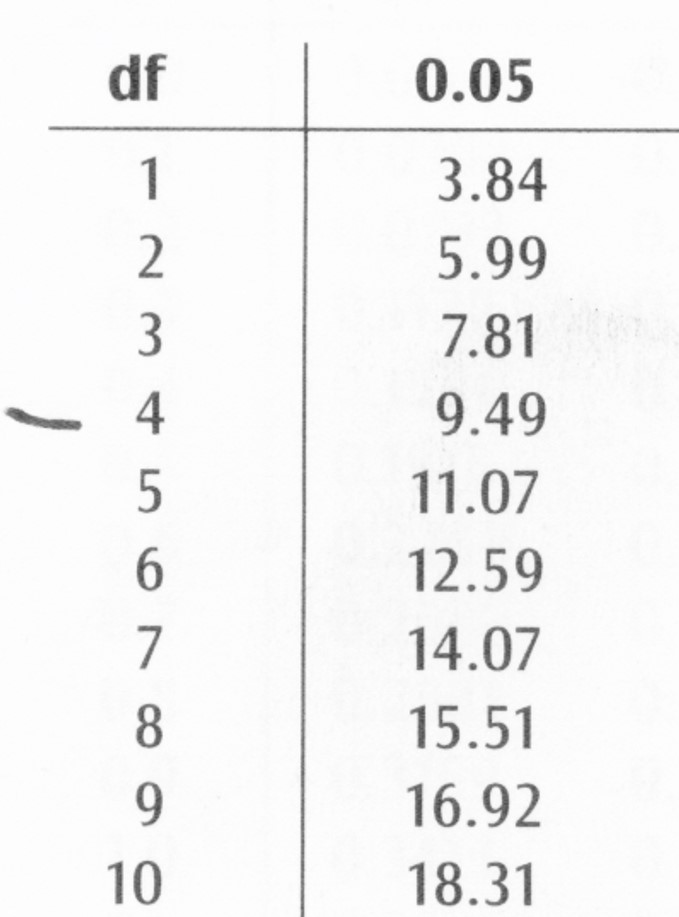
\includegraphics[height=1.4in]{chiTab.jpg}};
\end{tikzpicture}

\end{frame}

\begin{frame}{Associations - observed}
\protect\hypertarget{associations---observed}{}

\[ \chi^2 = \sum \frac{(O-E)^2}{E}\]

The observed values (\(O\)):

\begin{itemize}
\tightlist
\item
  the data we observe (obviously!)
\item
  cross tabulated counts
\end{itemize}

\end{frame}

\begin{frame}{Associations - expected}
\protect\hypertarget{associations---expected}{}

\[ \chi^2 = \sum \frac{(O-E)^2}{E}\]

The expected values (\(E\)):

\begin{itemize}
\tightlist
\item
  the data we would expect by change
\item
  the data we would expect if there was no association
\end{itemize}

\[E = \frac{\text{row total} \cdot \text{col total}}{\text{grand total}}\]

\end{frame}

\begin{frame}{Associations - expected}
\protect\hypertarget{associations---expected-1}{}

\[ \chi^2 = \sum \frac{(O-E)^2}{E}\]

Degrees of freedom:

\[ DF = (no. columns -1) \times (no. rows -1)\]

\end{frame}

\begin{frame}{Associations - expected}
\protect\hypertarget{associations---expected-2}{}

\[ \chi^2 = \sum \frac{(O-E)^2}{E}\]

\begin{tikzpicture}[remember picture,overlay]
\node[xshift=0cm,yshift=3.5cm] at (current page.south)
{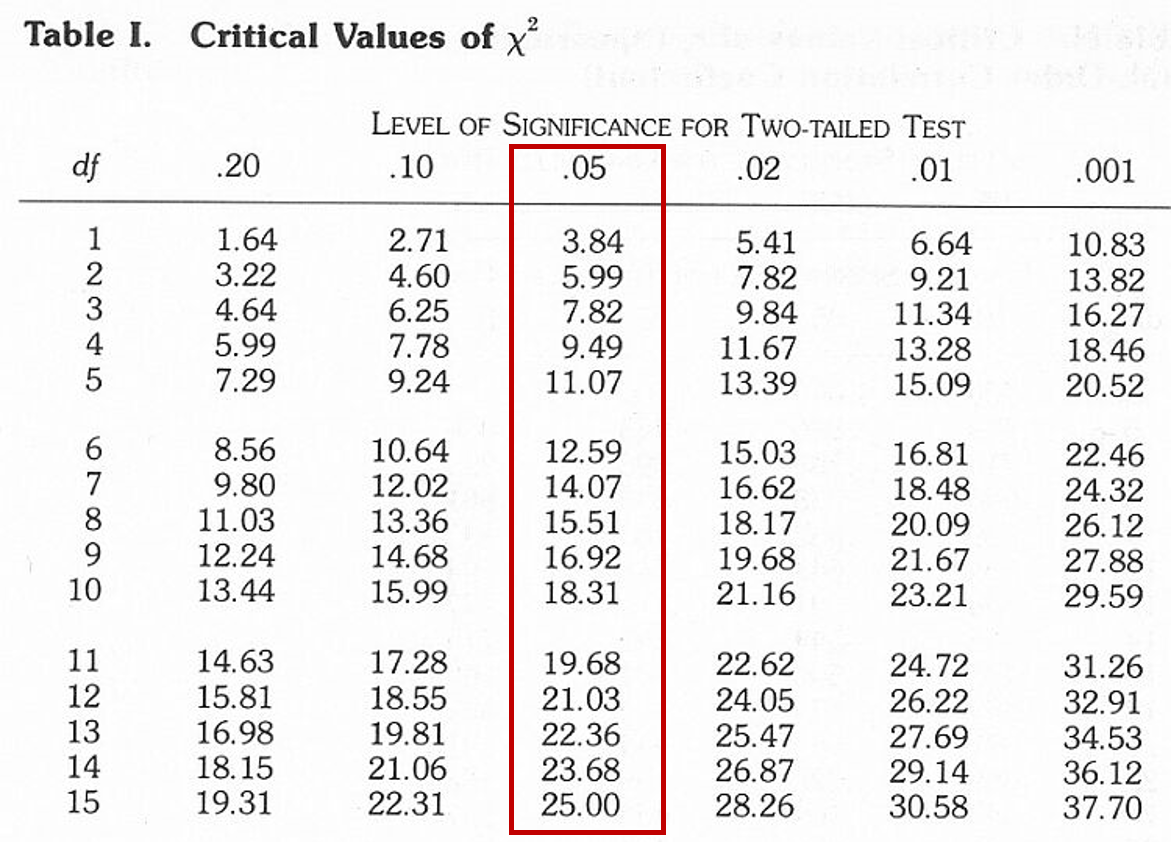
\includegraphics[height=2in]{chi5.png}};
\end{tikzpicture}

\end{frame}

\begin{frame}{Associations - invertebrate example}
\protect\hypertarget{associations---invertebrate-example}{}

Invertebrate group habitat selection:

\vfill

\centering

\begin{tabular}{lccc|c}
\toprule     
           & Ant & Bug  & Beetle & Total \\ \hline
Upper leaf & 15  &  13  & 68     &  96   \\   
Lower leaf & 12  &  11  & 15     &  38   \\   
Stem       & 65  &  78  &  5     & 148   \\   
Bud        &  3  &  21  &  3     &  27   \\ \hline    
Total      & 95  & 123  & 91     & 309   \\ \bottomrule    

\hline
\end{tabular}

\vfill

\end{frame}

\begin{frame}{Associations - invertebrate example}
\protect\hypertarget{associations---invertebrate-example-1}{}

First we need to state the hypotheses!

\begin{itemize}
\tightlist
\item
  Null hypothesis:
\end{itemize}

\begin{tikzpicture}[remember picture,overlay]
\node[xshift=0cm,yshift=5cm] at (current page.south)
{
\includegraphics[height=1.5in]{QM.png}};
\end{tikzpicture}

\end{frame}

\begin{frame}{Associations - invertebrate example}
\protect\hypertarget{associations---invertebrate-example-2}{}

First we need to state the hypotheses!

\begin{itemize}
\tightlist
\item
  Null hypothesis:
\item
  the \emph{no habitat preference} hypothesis
\item
  random!
\end{itemize}

``There is no association between invertebrate group and habitat''

\end{frame}

\begin{frame}{Associations - invertebrate example}
\protect\hypertarget{associations---invertebrate-example-3}{}

First we need to state the hypotheses!

\begin{itemize}
\tightlist
\item
  Null hypothesis:
\item
  the \emph{no habitat preference} hypothesis
\item
  random!
\end{itemize}

``There is no association between invertebrate group and habitat''

\vspace{0.5cm}

\begin{itemize}
\tightlist
\item
  Alternative hypothesis:
\end{itemize}

\begin{tikzpicture}[remember picture,overlay]
\node[xshift=0cm,yshift=2cm] at (current page.south)
{
\includegraphics[height=1.5in]{QM.png}};
\end{tikzpicture}

\end{frame}

\begin{frame}{Associations - invertebrate example}
\protect\hypertarget{associations---invertebrate-example-4}{}

First we need to state the hypotheses!

\begin{itemize}
\tightlist
\item
  Null hypothesis:
\item
  the \emph{no habitat preference} hypothesis
\item
  random!
\end{itemize}

``There is no association between invertebrate group and habitat''

\vspace{0.25cm}

\begin{itemize}
\tightlist
\item
  Alternative hypothesis:
\item
  the \emph{habitat preference} hypothesis

  \begin{itemize}
  \tightlist
  \item
    direction not explicitly stated
  \item
    can be positive or negative
  \end{itemize}
\item
  not random!
\end{itemize}

``There \emph{is} an association between invertebrate group and
habitat''

\end{frame}

\begin{frame}{Associations - invertebrate example}
\protect\hypertarget{associations---invertebrate-example-5}{}

\vfill
\centering
\Large

Demo in \texttt{Excel}

\vfill

\end{frame}

\begin{frame}{Associations - invertebrate example}
\protect\hypertarget{associations---invertebrate-example-6}{}

\begin{itemize}
\tightlist
\item
  The test statistic is \(\chi^2 = 146.98\).
\item
  What do we conclude?
\end{itemize}

\end{frame}

\begin{frame}{Associations - invertebrate example}
\protect\hypertarget{associations---invertebrate-example-7}{}

\begin{itemize}
\tightlist
\item
  The test statistic is \(\chi^2 = 146.98\).
\item
  What do we conclude?

  \begin{itemize}
  \tightlist
  \item
    \(p < 0.05\)
  \item
    reject the null hypothesis
  \item
    accept the alternative hypothesis
  \item
    there \emph{is} a significant association between inverts and
    habitat!
  \end{itemize}
\end{itemize}

\end{frame}

\begin{frame}{Associations - invertebrate example}
\protect\hypertarget{associations---invertebrate-example-8}{}

\begin{itemize}
\tightlist
\item
  The test statistic is \(\chi^2 = 146.98\).
\item
  What do we conclude?

  \begin{itemize}
  \tightlist
  \item
    \(p < 0.05\)
  \item
    reject the null hypothesis
  \item
    accept the alternative hypothesis
  \item
    there \emph{is} a significant association between inverts and
    habitat!
  \end{itemize}
\item
  BUT! which associations are significant?
\end{itemize}

\centering

\begin{tabular}{lcccc}
\toprule     
           & Ant & Bug  & Beetle & Total \\ \hline
Upper leaf & 15  &  13  & 68     &  96   \\   
Lower leaf & 12  &  11  & 15     &  38   \\   
Stem       & 65  &  78  &  5     & 148   \\   
Bud        &  3  &  21  &  3     &  27   \\ \hline    
Total      & 95  & 123  & 91     & 309   \\ \bottomrule    

\hline
\end{tabular}

\end{frame}

\begin{frame}{Associations - significant associations}
\protect\hypertarget{associations---significant-associations}{}

Two ways we can evaluate which associations are likely to be
significant:

\begin{enumerate}
\tightlist
\item
  Cell-specific \(\chi^2\) values

  \begin{itemize}
  \tightlist
  \item
    greater than 3.8 is likely to be significant
  \item
    3.8 is significant test statistic with 1 degree of freedom
  \end{itemize}
\end{enumerate}

\end{frame}

\begin{frame}{Associations - significant associations}
\protect\hypertarget{associations---significant-associations-1}{}

Two ways we can evaluate which associations are likely to be
significant:

\begin{enumerate}
\tightlist
\item
  Cell-specific \(\chi^2\) values

  \begin{itemize}
  \tightlist
  \item
    greater than 3.8 is likely to be significant
  \item
    3.8 is significant test statistic with 1 degree of freedom
  \end{itemize}
\item
  Pearson residuals

  \begin{itemize}
  \tightlist
  \item
    provides sign of association
  \item
    provides relative size of the association
  \item
    if residual is \textgreater2 or \textless{} -2 then likely to be
    significant
  \end{itemize}
\end{enumerate}

\[ Residual = \frac{\text{Observed}-\text{Expected}}{\sqrt{\text{Expected}}}\]

\end{frame}

\begin{frame}{Associations - invertebrate example}
\protect\hypertarget{associations---invertebrate-example-9}{}

\vfill
\centering
\Large

Back to \texttt{Excel}

\vfill

\end{frame}

\begin{frame}[fragile]{Analyzing contingency table data in
\texttt{Excel}}
\protect\hypertarget{analyzing-contingency-table-data-in}{}

Two \texttt{Excel} functions for doing Chi-squared or Goodness of fit
tests but no method in \emph{Analysis Tool Pack}:

\end{frame}

\begin{frame}[fragile]{Analyzing contingency table data in
\texttt{Excel}}
\protect\hypertarget{analyzing-contingency-table-data-in-1}{}

Two \texttt{Excel} functions for doing Chi-squared or Goodness of fit
tests but no method in \emph{Analysis Tool Pack}:

\begin{itemize}
\tightlist
\item
  \texttt{CHITEST(}\emph{observed},\emph{expected}\texttt{)}

  \begin{itemize}
  \tightlist
  \item
    must calculate the \emph{expected} values
  \item
    must be in the same table format
  \end{itemize}
\end{itemize}

\end{frame}

\begin{frame}[fragile]{Analyzing contingency table data in
\texttt{Excel}}
\protect\hypertarget{analyzing-contingency-table-data-in-2}{}

Two \texttt{Excel} functions for doing Chi-squared or Goodness of fit
tests but no method in \emph{Analysis Tool Pack}:

\begin{itemize}
\tightlist
\item
  \texttt{CHITEST(}\emph{observed},\emph{expected}\texttt{)}

  \begin{itemize}
  \tightlist
  \item
    must calculate the \emph{expected} values
  \item
    must be in the same table format
  \end{itemize}
\item
  \texttt{CHIDIST(}\emph{Chi value},\emph{derees of freedom}\texttt{)}

  \begin{itemize}
  \tightlist
  \item
    must calculate \(\chi^2\) and DF
  \item
    just calculates a \emph{p}-value
  \end{itemize}
\end{itemize}

\vfill
\centering

Demo in \texttt{Excel}

\vfill

\end{frame}

\begin{frame}[fragile]{Analyzing contingency table data in \texttt{R}}
\protect\hypertarget{analyzing-contingency-table-data-in-3}{}

\begin{itemize}
\tightlist
\item
  Chi-square test in \texttt{R}

  \begin{itemize}
  \tightlist
  \item
    \texttt{chisq.test(}\emph{contingency table}\texttt{)}
  \item
    data must be formatted like a contingency table
  \item
    can make a \texttt{data.frame}
  \end{itemize}
\end{itemize}

\scriptsize

\begin{Shaded}
\begin{Highlighting}[]
\CommentTok{# a dataframe}
\NormalTok{tab.df <-}\StringTok{ }\KeywordTok{data.frame}\NormalTok{(}\DataTypeTok{Ant =} \KeywordTok{c}\NormalTok{(}\DecValTok{15}\NormalTok{,}\DecValTok{12}\NormalTok{,}\DecValTok{65}\NormalTok{,}\DecValTok{3}\NormalTok{),}
                     \DataTypeTok{Bug =} \KeywordTok{c}\NormalTok{(}\DecValTok{13}\NormalTok{,}\DecValTok{11}\NormalTok{,}\DecValTok{78}\NormalTok{,}\DecValTok{21}\NormalTok{),}
                     \DataTypeTok{Beetle =} \KeywordTok{c}\NormalTok{(}\DecValTok{68}\NormalTok{,}\DecValTok{15}\NormalTok{,}\DecValTok{5}\NormalTok{,}\DecValTok{3}\NormalTok{))}
\KeywordTok{rownames}\NormalTok{(tab.df) <-}\StringTok{ }\KeywordTok{c}\NormalTok{(}\StringTok{"Upper"}\NormalTok{, }\StringTok{"Lower"}\NormalTok{, }\StringTok{"Stem"}\NormalTok{, }\StringTok{"Bud"}\NormalTok{)}
\NormalTok{tab.df}
\NormalTok{      Ant Bug Beetle}
\NormalTok{Upper  }\DecValTok{15}  \DecValTok{13}     \DecValTok{68}
\NormalTok{Lower  }\DecValTok{12}  \DecValTok{11}     \DecValTok{15}
\NormalTok{Stem   }\DecValTok{65}  \DecValTok{78}      \DecValTok{5}
\NormalTok{Bud     }\DecValTok{3}  \DecValTok{21}      \DecValTok{3}
\end{Highlighting}
\end{Shaded}

\end{frame}

\begin{frame}[fragile]{Analyzing contingency table data in \texttt{R}}
\protect\hypertarget{analyzing-contingency-table-data-in-4}{}

\begin{itemize}
\tightlist
\item
  Chi-square test in \texttt{R}

  \begin{itemize}
  \tightlist
  \item
    \texttt{chisq.test(}\emph{contingency table}\texttt{)}
  \item
    data must be formatted like a contingency table
  \item
    can make a \texttt{matrix}
  \end{itemize}
\end{itemize}

\scriptsize

\begin{Shaded}
\begin{Highlighting}[]
\CommentTok{# a dataframe}
\NormalTok{tab.mat <-}\StringTok{ }\KeywordTok{matrix}\NormalTok{(}\KeywordTok{c}\NormalTok{(}\DecValTok{15}\NormalTok{,}\DecValTok{12}\NormalTok{,}\DecValTok{65}\NormalTok{,}\DecValTok{3}\NormalTok{,}
                    \DecValTok{13}\NormalTok{,}\DecValTok{11}\NormalTok{,}\DecValTok{78}\NormalTok{,}\DecValTok{21}\NormalTok{,}
                    \DecValTok{68}\NormalTok{,}\DecValTok{15}\NormalTok{,}\DecValTok{5}\NormalTok{,}\DecValTok{3}\NormalTok{), }\DataTypeTok{nrow=}\DecValTok{4}\NormalTok{, }\DataTypeTok{ncol=}\DecValTok{3}\NormalTok{, }\DataTypeTok{byrow=}\OtherTok{FALSE}\NormalTok{)}
\KeywordTok{rownames}\NormalTok{(tab.mat) <-}\StringTok{ }\KeywordTok{c}\NormalTok{(}\StringTok{"Upper"}\NormalTok{, }\StringTok{"Lower"}\NormalTok{, }\StringTok{"Stem"}\NormalTok{, }\StringTok{"Bud"}\NormalTok{)}
\KeywordTok{colnames}\NormalTok{(tab.mat) <-}\StringTok{ }\KeywordTok{c}\NormalTok{(}\StringTok{"Ant"}\NormalTok{, }\StringTok{"Bug"}\NormalTok{, }\StringTok{"Beetle"}\NormalTok{)}
\NormalTok{tab.mat}
\NormalTok{      Ant Bug Beetle}
\NormalTok{Upper  }\DecValTok{15}  \DecValTok{13}     \DecValTok{68}
\NormalTok{Lower  }\DecValTok{12}  \DecValTok{11}     \DecValTok{15}
\NormalTok{Stem   }\DecValTok{65}  \DecValTok{78}      \DecValTok{5}
\NormalTok{Bud     }\DecValTok{3}  \DecValTok{21}      \DecValTok{3}
\end{Highlighting}
\end{Shaded}

\end{frame}

\begin{frame}[fragile]{Analyzing contingency table data in
\texttt{Excel}}
\protect\hypertarget{analyzing-contingency-table-data-in-5}{}

\begin{itemize}
\tightlist
\item
  Chi-square test in \texttt{R}

  \begin{itemize}
  \tightlist
  \item
    \texttt{chisq.test(}\emph{contingency table}\texttt{)}
  \item
    data must be formatted like a contingency table
  \item
    can make a \texttt{data.frame} or a \texttt{matrix}
  \end{itemize}
\end{itemize}

\scriptsize

\begin{Shaded}
\begin{Highlighting}[]
\CommentTok{# conduct the Chi-square test}
\KeywordTok{chisq.test}\NormalTok{(tab.df)}

\NormalTok{    Pearson}\StringTok{'s Chi-squared test}

\StringTok{data:  tab.df}
\StringTok{X-squared = 146.98, df = 6, p-value < 2.2e-16}
\end{Highlighting}
\end{Shaded}

\end{frame}

\begin{frame}[fragile]{Analyzing contingency table data in
\texttt{Excel}}
\protect\hypertarget{analyzing-contingency-table-data-in-6}{}

\begin{itemize}
\tightlist
\item
  Chi-square test in \texttt{R}

  \begin{itemize}
  \tightlist
  \item
    \texttt{chisq.test(}\emph{contingency table}\texttt{)}
  \item
    data must be formatted like a contingency table
  \item
    can make a \texttt{data.frame} or a \texttt{matrix}
  \end{itemize}
\end{itemize}

\scriptsize

\begin{Shaded}
\begin{Highlighting}[]
\CommentTok{# extract the expected values}
\KeywordTok{chisq.test}\NormalTok{(tab.df)}\OperatorTok{$}\NormalTok{expected}
\NormalTok{            Ant      Bug    Beetle}
\NormalTok{Upper }\FloatTok{29.514563} \FloatTok{38.21359} \FloatTok{28.271845}
\NormalTok{Lower }\FloatTok{11.682848} \FloatTok{15.12621} \FloatTok{11.190939}
\NormalTok{Stem  }\FloatTok{45.501618} \FloatTok{58.91262} \FloatTok{43.585761}
\NormalTok{Bud    }\FloatTok{8.300971} \FloatTok{10.74757}  \FloatTok{7.951456}
\end{Highlighting}
\end{Shaded}

\end{frame}

\begin{frame}[fragile]{Analyzing contingency table data in
\texttt{Excel}}
\protect\hypertarget{analyzing-contingency-table-data-in-7}{}

\begin{itemize}
\tightlist
\item
  Chi-square test in \texttt{R}

  \begin{itemize}
  \tightlist
  \item
    \texttt{chisq.test(}\emph{contingency table}\texttt{)}
  \item
    data must be formatted like a contingency table
  \item
    can make a \texttt{data.frame} or a \texttt{matrix}
  \end{itemize}
\end{itemize}

\scriptsize

\begin{Shaded}
\begin{Highlighting}[]
\CommentTok{# calculate the Pearson residuals}
\NormalTok{obs <-}\StringTok{ }\NormalTok{tab.df}
\NormalTok{exp <-}\StringTok{ }\KeywordTok{chisq.test}\NormalTok{(tab.df)}\OperatorTok{$}\NormalTok{expected}
\NormalTok{(obs}\OperatorTok{-}\NormalTok{exp) }\OperatorTok{/}\StringTok{ }\KeywordTok{sqrt}\NormalTok{(exp)}
\NormalTok{             Ant       Bug    Beetle}
\NormalTok{Upper }\FloatTok{-2.6716883} \FloatTok{-4.078738}  \FloatTok{7.471733}
\NormalTok{Lower  }\FloatTok{0.0927883} \FloatTok{-1.060930}  \FloatTok{1.138636}
\NormalTok{Stem   }\FloatTok{2.8905810}  \FloatTok{2.486807} \FloatTok{-5.844599}
\NormalTok{Bud   }\FloatTok{-1.8398862}  \FloatTok{3.127314} \FloatTok{-1.755940}
\end{Highlighting}
\end{Shaded}

\end{frame}

\begin{frame}[fragile]{Analyzing contingency table data in
\texttt{Excel}}
\protect\hypertarget{analyzing-contingency-table-data-in-8}{}

What can we conclude from our analysis of the invertebrate data using
the Chi-square test for association?\\
\scriptsize

\begin{Shaded}
\begin{Highlighting}[]
\CommentTok{# conduct the Chi-square test}
\KeywordTok{chisq.test}\NormalTok{(tab.df)}

\NormalTok{    Pearson}\StringTok{'s Chi-squared test}

\StringTok{data:  tab.df}
\StringTok{X-squared = 146.98, df = 6, p-value < 2.2e-16}
\end{Highlighting}
\end{Shaded}

\begin{Shaded}
\begin{Highlighting}[]
\CommentTok{# Pearson residuals}
\NormalTok{(obs}\OperatorTok{-}\NormalTok{exp) }\OperatorTok{/}\StringTok{ }\KeywordTok{sqrt}\NormalTok{(exp)}
\NormalTok{             Ant       Bug    Beetle}
\NormalTok{Upper }\FloatTok{-2.6716883} \FloatTok{-4.078738}  \FloatTok{7.471733}
\NormalTok{Lower  }\FloatTok{0.0927883} \FloatTok{-1.060930}  \FloatTok{1.138636}
\NormalTok{Stem   }\FloatTok{2.8905810}  \FloatTok{2.486807} \FloatTok{-5.844599}
\NormalTok{Bud   }\FloatTok{-1.8398862}  \FloatTok{3.127314} \FloatTok{-1.755940}
\end{Highlighting}
\end{Shaded}

\end{frame}

\begin{frame}{`Pioneer Valley Camera Trapping Data'}
\protect\hypertarget{pioneer-valley-camera-trapping-data}{}

The data:

\begin{itemize}
\tightlist
\item
  142 camera traps placed throughout the valley
\item
  each camera has 2 categorical covariates:

  \begin{itemize}
  \tightlist
  \item
    land use: `altered' (A), `natural' (N) and `urban' (U)
  \item
    scent lure: `Badlands Bob' (BB) and `Powder River' (PR)
  \end{itemize}
\item
  we will focus on four species:

  \begin{itemize}
  \tightlist
  \item
    bobcat \emph{lynx rufus}
  \item
    domestic cat \emph{felis catus}
  \item
    coyote \emph{canis latrans}
  \item
    domestic dog \emph{canis familiaris}
  \end{itemize}
\end{itemize}

\end{frame}

\begin{frame}{Group exercise}
\protect\hypertarget{group-exercise}{}

Using the `Pioneer Valley Camera Trapping Data' investigate whether
there is a statistically significant association between the four
species and:

\begin{enumerate}
\tightlist
\item
  habitat type
\item
  scent lure
\end{enumerate}

(i.e., conduct two analyses)

\begin{tikzpicture}[remember picture,overlay]
\node[xshift=0cm,yshift=2.5cm] at (current page.south)
{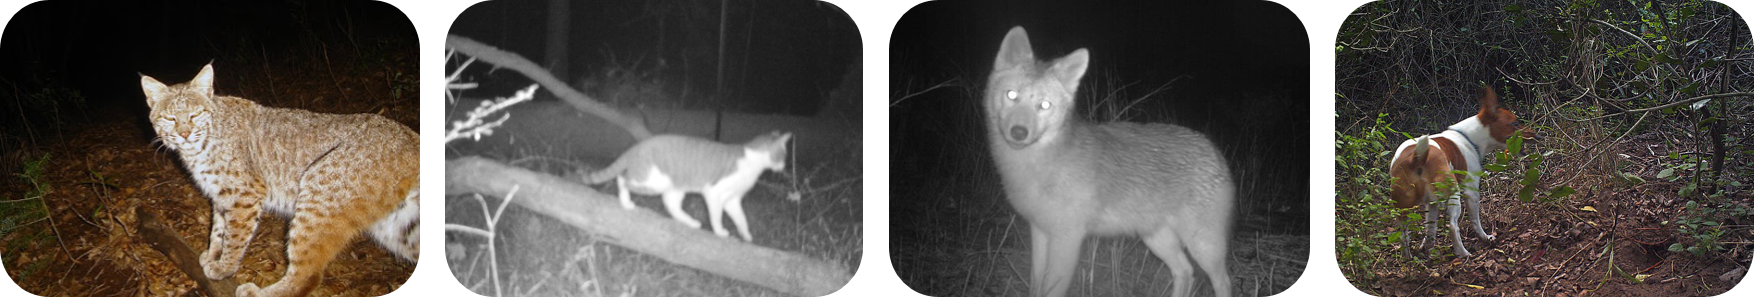
\includegraphics[height=0.8in]{camtraps.png}};
\end{tikzpicture}

\end{frame}

\end{document}
